\chapter{Imágenes analizadas con Google Cloud Vision \acs{API}}
\label{chap:imagenes}

\drop{E}{}n este anexo se reflejan las imágenes del caso de estudio 2, tanto las que tienen que ver con la estación de control terrestre como las pertenecientes al \textit{Módulo de Análisis de Imágenes}. También, se presentan un conjunto de imágenes, con sus resultados, al realizar el análisis con vídeos extraídos de internet.

\section{Imágenes del caso de estudio 2}

\subsection{Estación de control terrestre}

\begin{figure}[!h]
\begin{center}
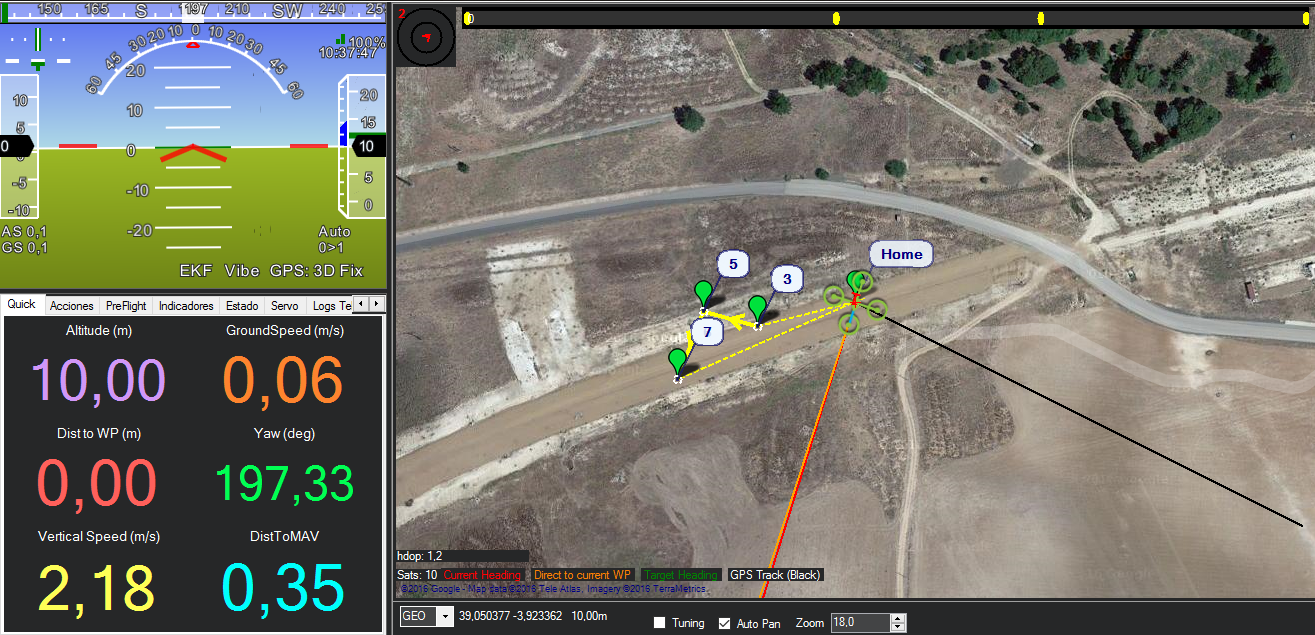
\includegraphics[width=1\textwidth]{/0.png}
\caption[Despegue del 3DR IRIS+]{Despegue del 3DR IRIS+}
\label{fig:despegue1}
\end{center}
\end{figure}

\begin{figure}[!h]
\begin{center}
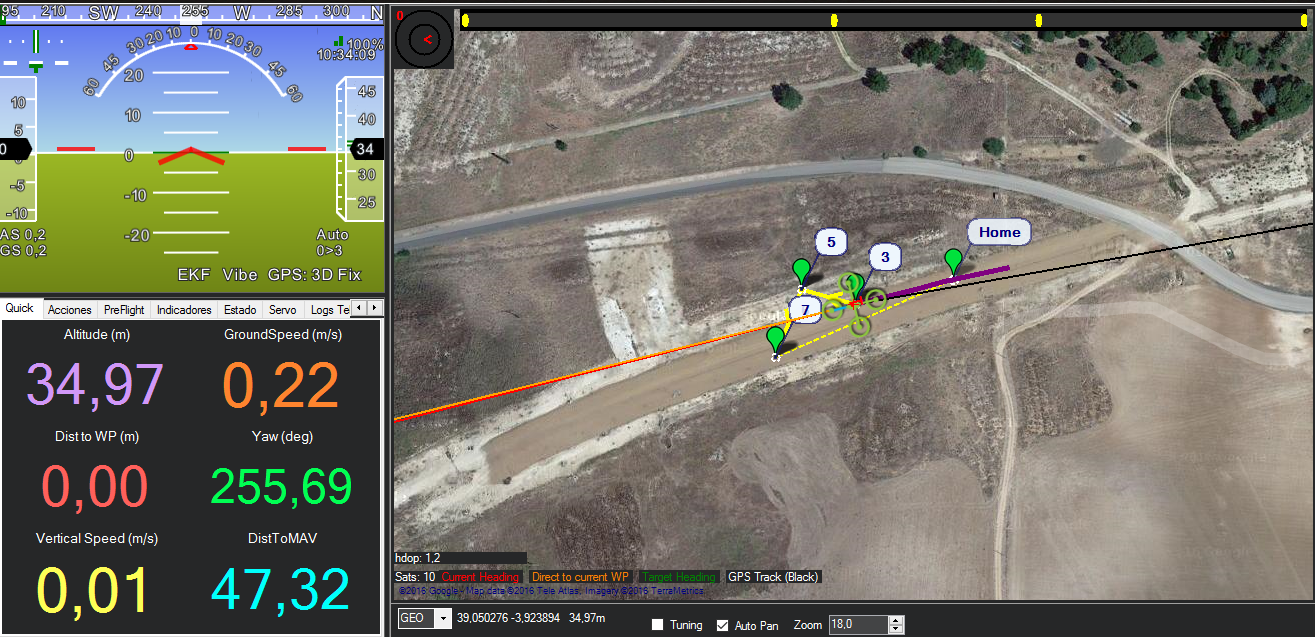
\includegraphics[width=1\textwidth]{/1.png}
\caption[3DR IRIS+ volando a «waypoint» 1]{3DR IRIS+ volando a «waypoint» 1}
\label{fig:despegue2}
\end{center}
\end{figure}

\begin{figure}[!h]
\begin{center}
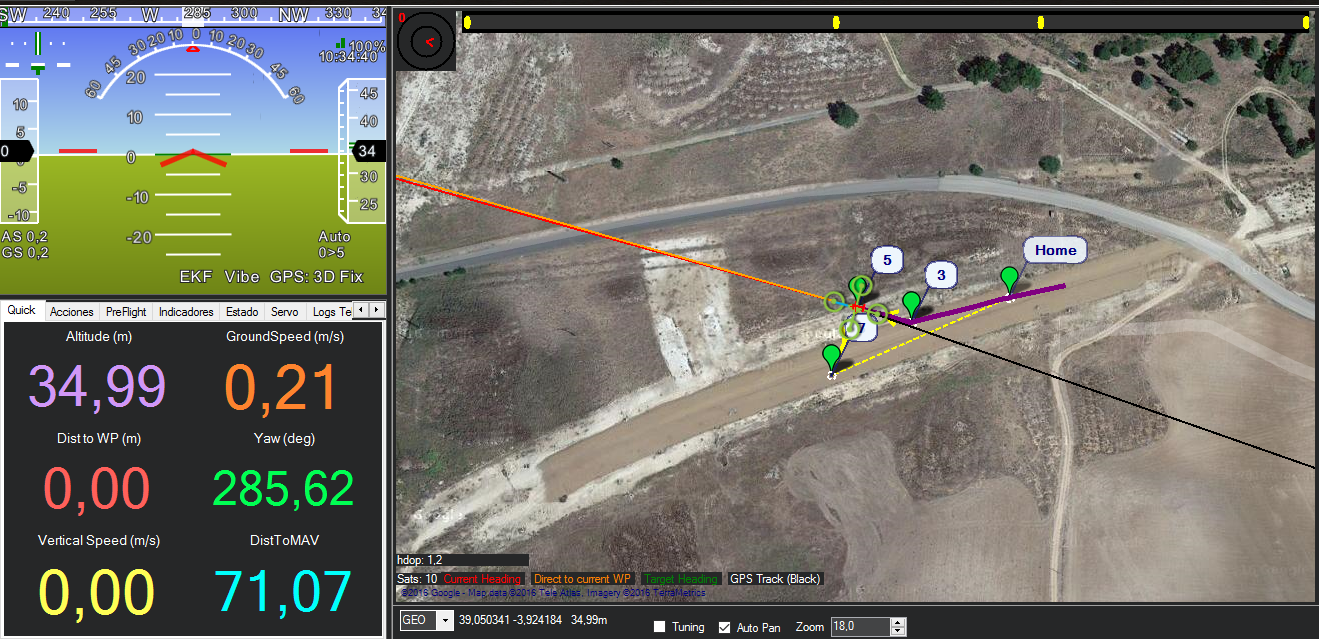
\includegraphics[width=1\textwidth]{/2.png}
\caption[3DR IRIS+ volando a «waypoint» 2]{3DR IRIS+ volando a «waypoint» 2}
\label{fig:despegue3}
\end{center}
\end{figure}

\begin{figure}[!h]
\begin{center}
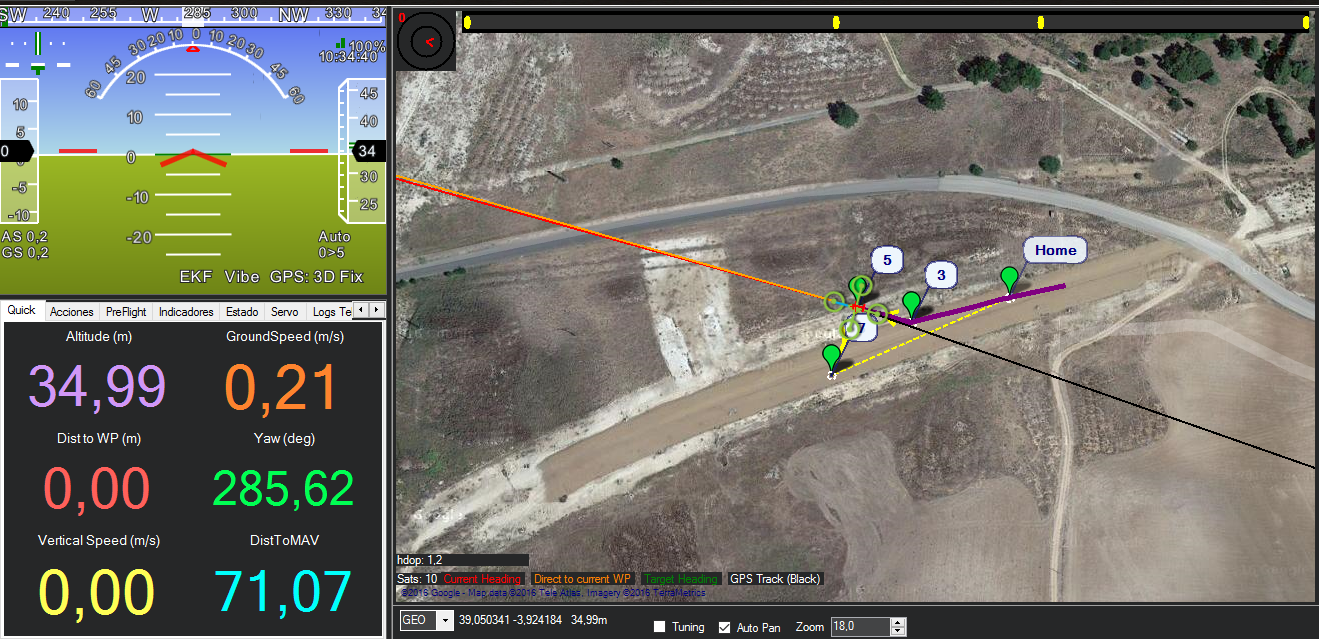
\includegraphics[width=1\textwidth]{/2.png}
\caption[3DR IRIS+ volando a «waypoint» 3]{3DR IRIS+ volando a «waypoint» 3}
\label{fig:despegue4}
\end{center}
\end{figure}

\begin{figure}[!h]
\begin{center}
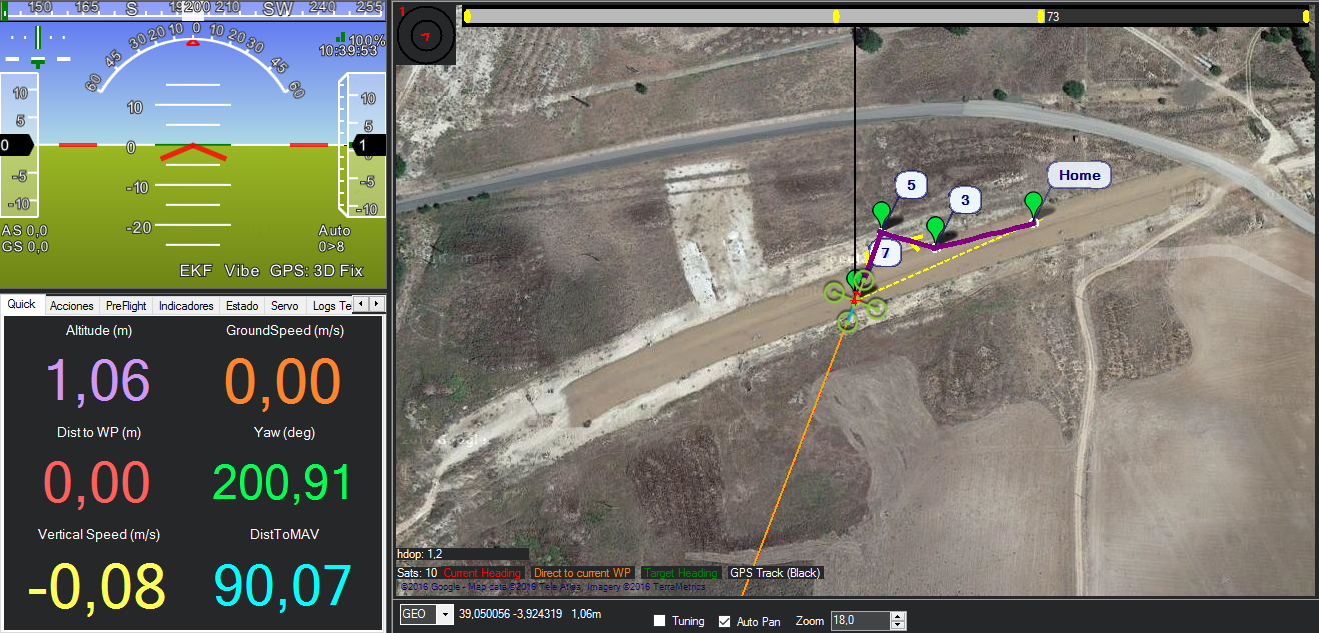
\includegraphics[width=1\textwidth]{/00.png}
\caption[3DR IRIS+ realizando el aterrizaje]{3DR IRIS+ realizando el aterrizaje}
\label{fig:despegue5}
\end{center}
\end{figure}

\clearpage

\subsection{Imágenes analizadas}

\begin{figure}[!h]
\begin{center}
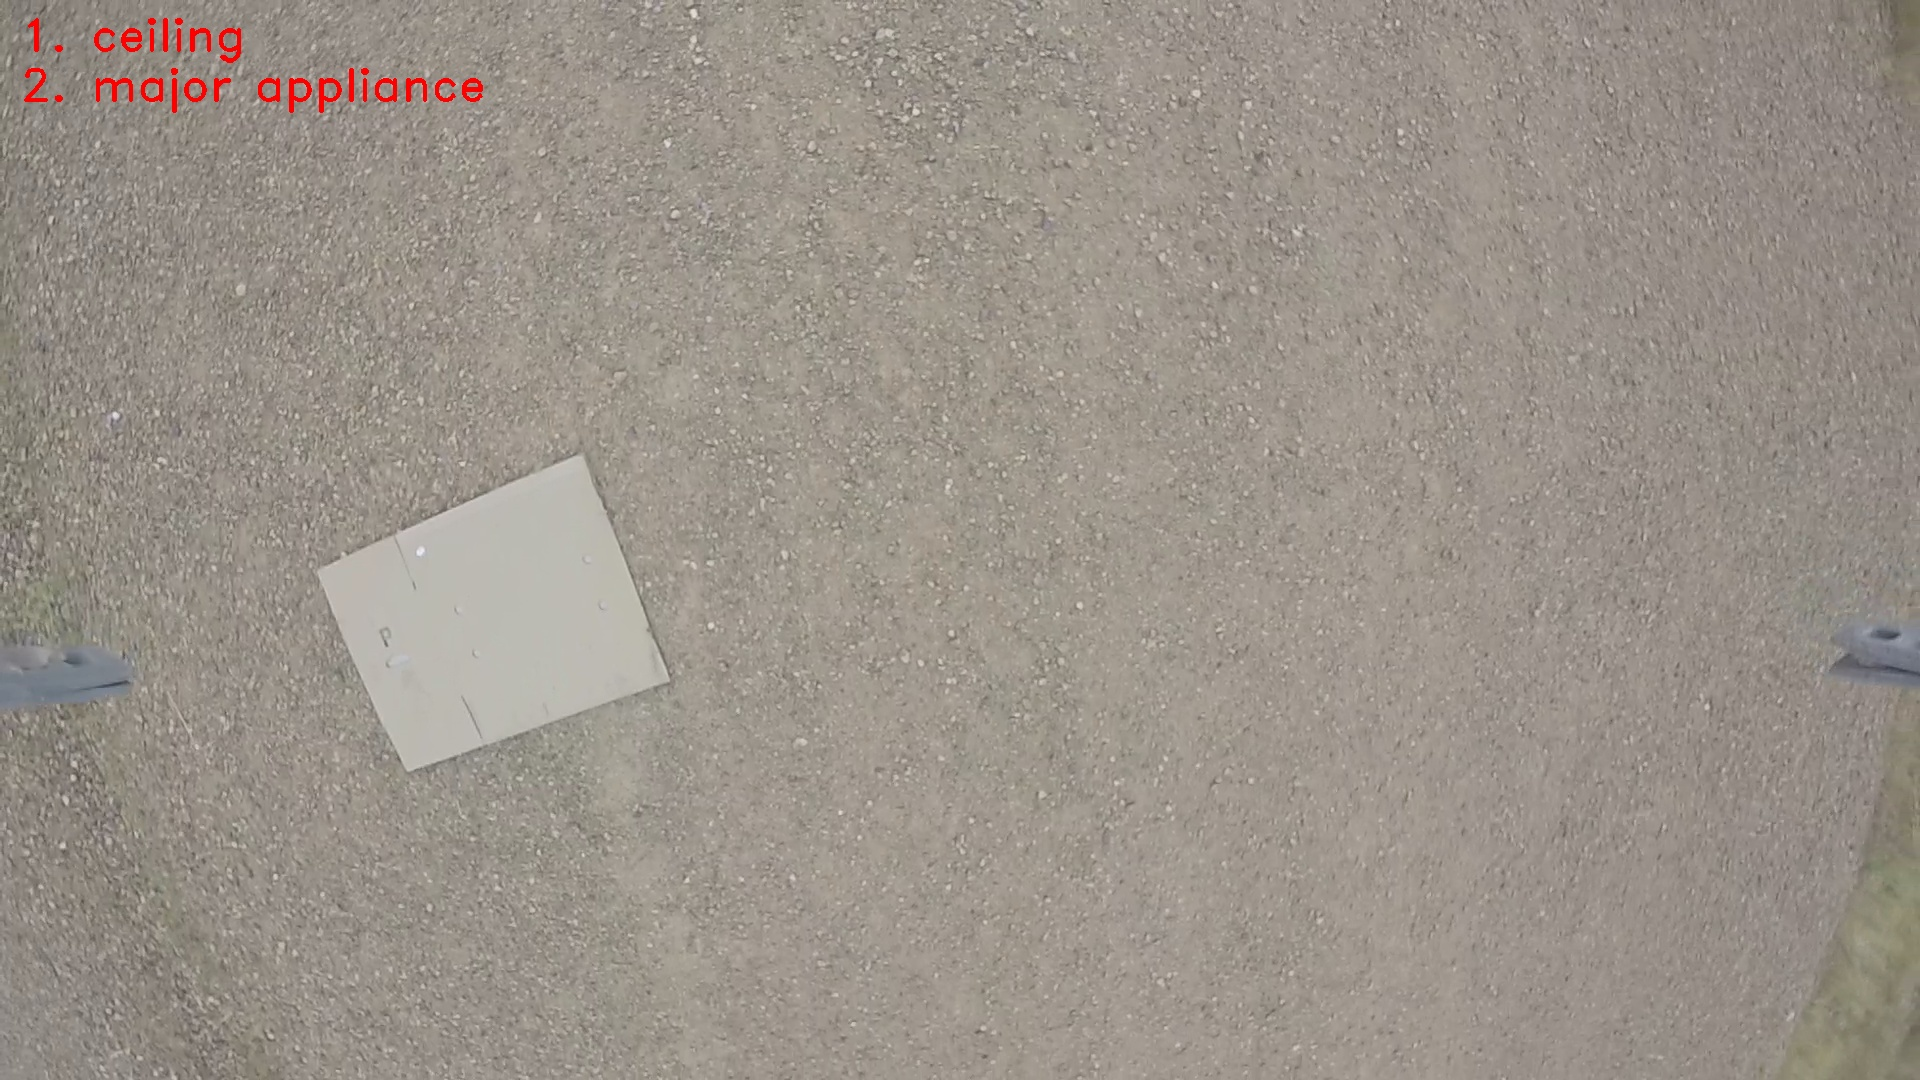
\includegraphics[width=1\textwidth]{/11.jpg}
\caption[Análisis de imagen durante despegue]{Análisis de imagen durante despegue}
\label{fig:imagen11}
\end{center}
\end{figure}

\begin{figure}[!h]
\begin{center}
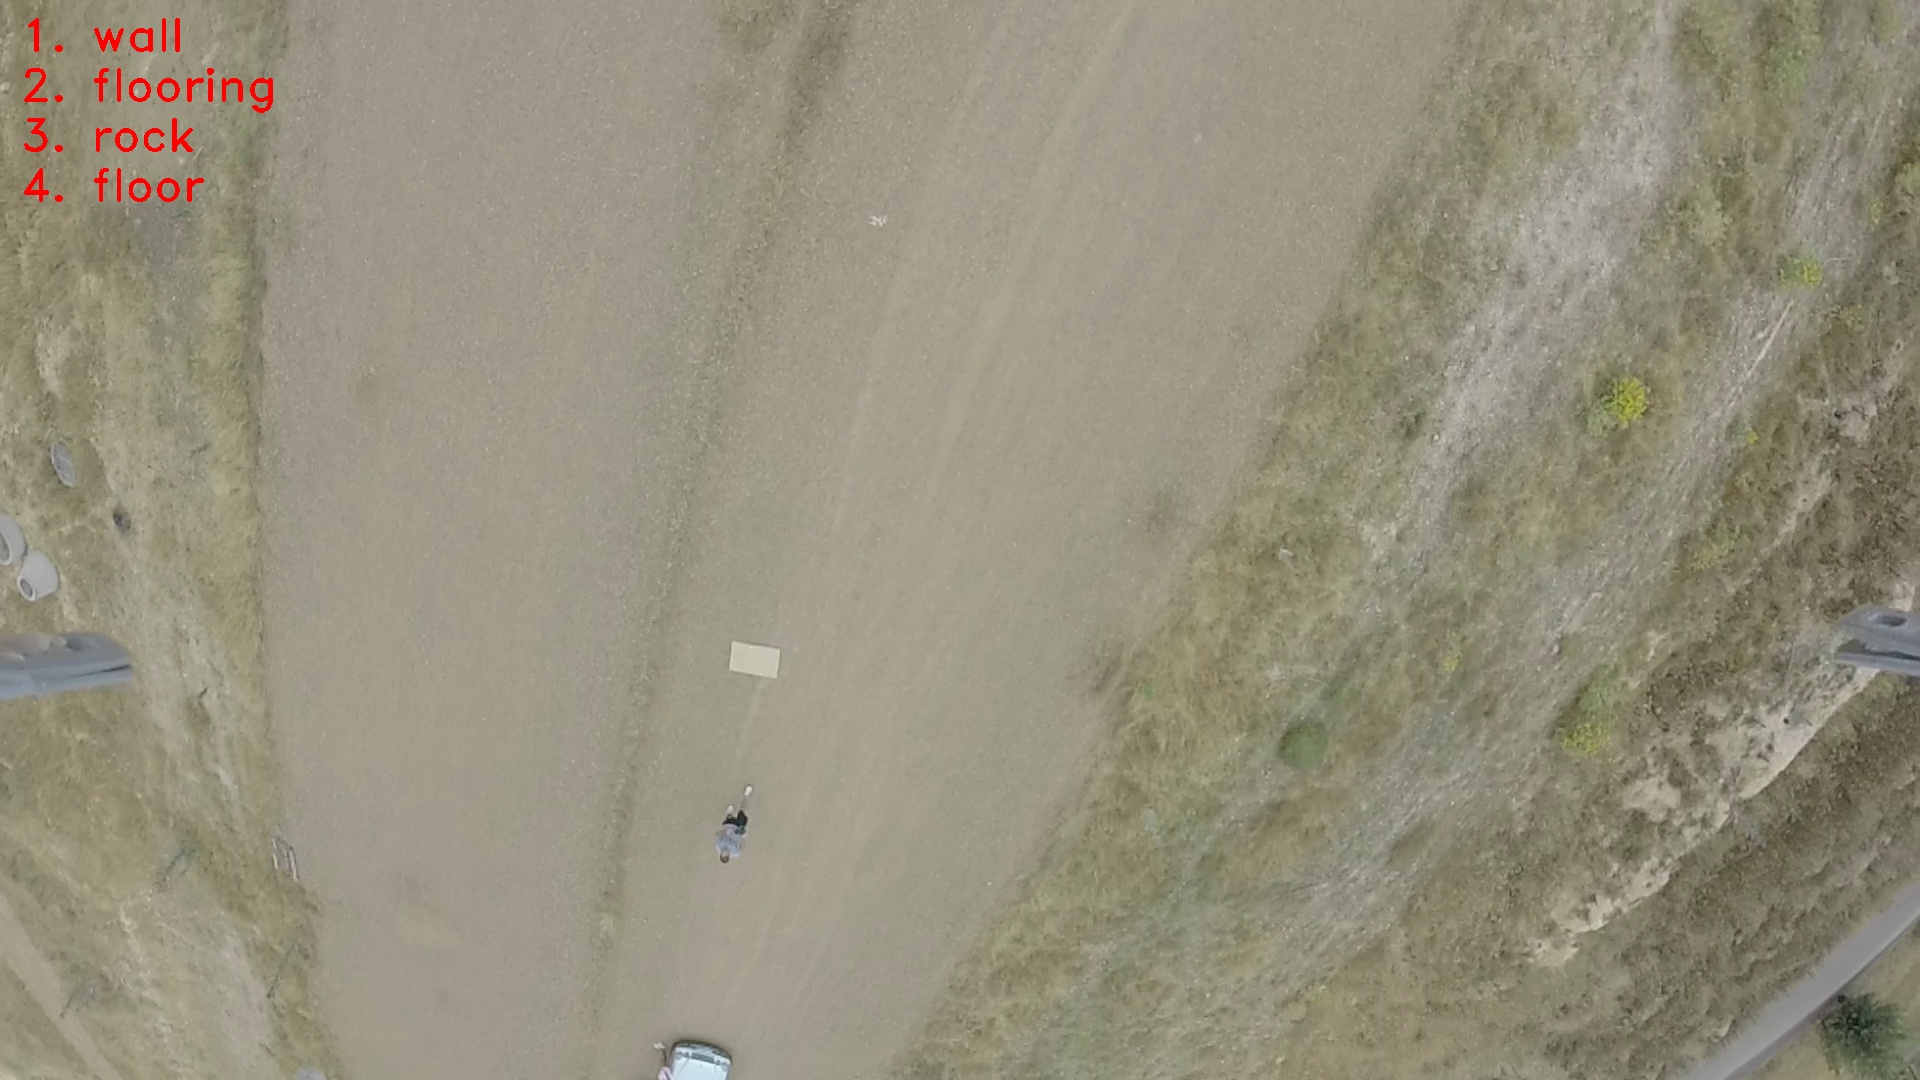
\includegraphics[width=1\textwidth]{/12.jpg}
\caption[Análisis de imagen al llegar al «waypoint» 1]{Análisis de imagen al llegar al «waypoint» 1}
\label{fig:imagen2}
\end{center}
\end{figure}

\begin{figure}[!h]
\begin{center}
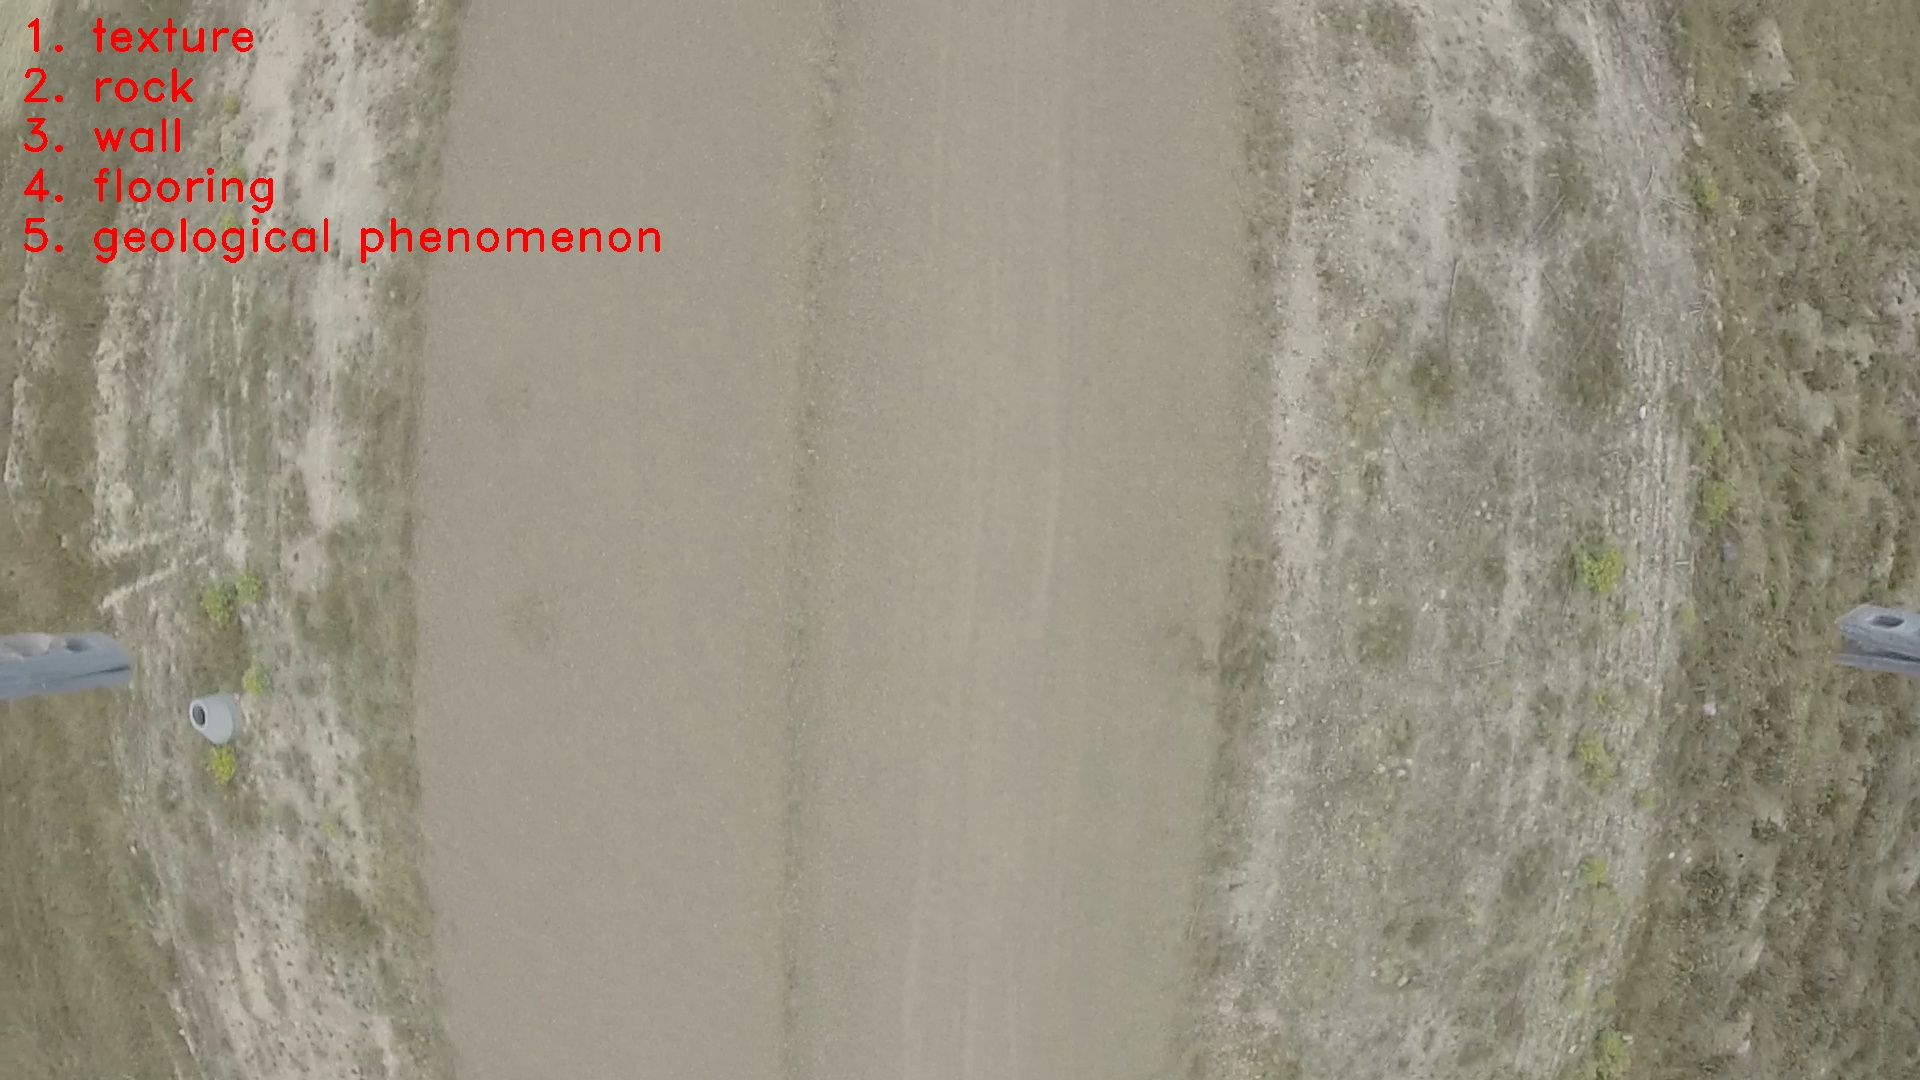
\includegraphics[width=1\textwidth]{/13.jpg}
\caption[Análisis de imagen al llegar al «waypoint» 2]{Análisis de imagen al llegar al «waypoint» 2}
\label{fig:imagen3}
\end{center}
\end{figure}

\begin{figure}[!h]
\begin{center}
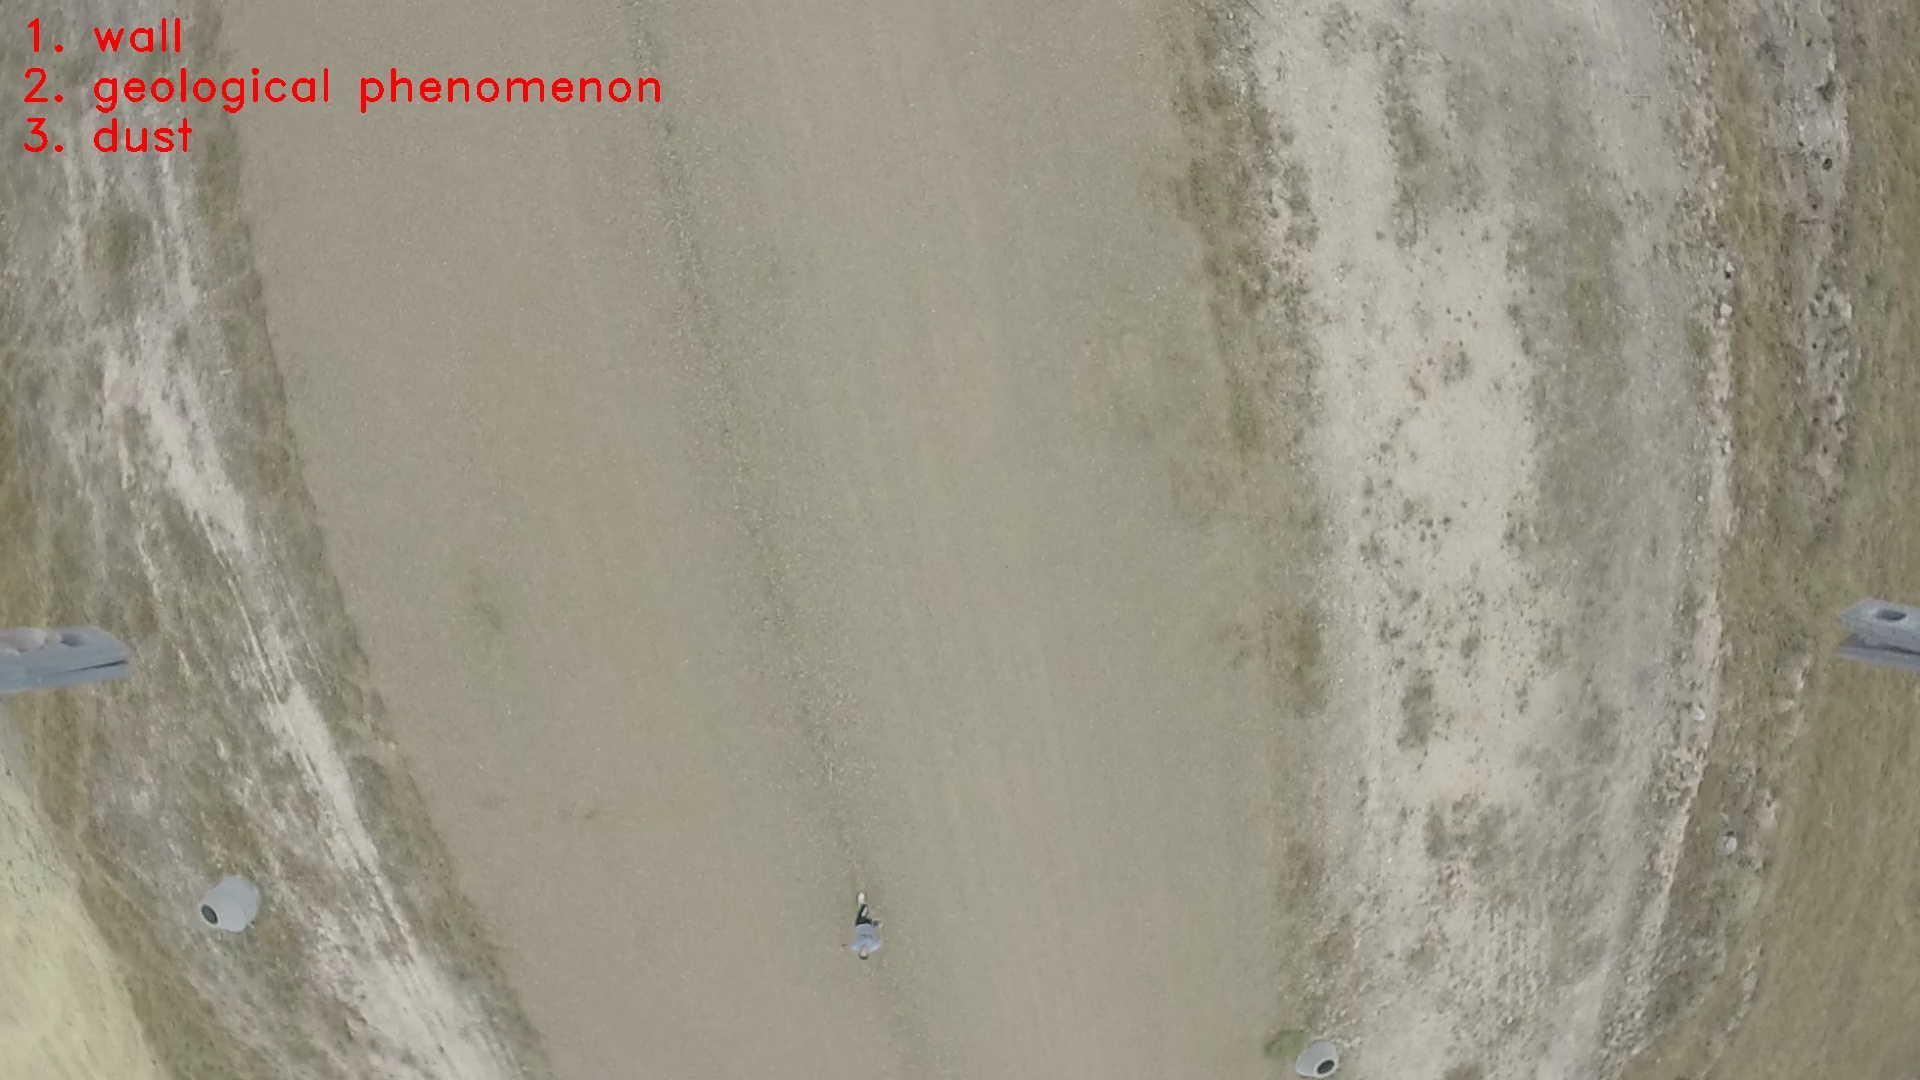
\includegraphics[width=1\textwidth]{/14.jpg}
\caption[Análisis de imagen al llegar al «waypoint» 3]{Análisis de imagen al llegar al «waypoint» 3}
\label{fig:imagen4}
\end{center}
\end{figure}

\clearpage

\section{Otras imágenes}

\begin{figure}[!h]
\begin{center}
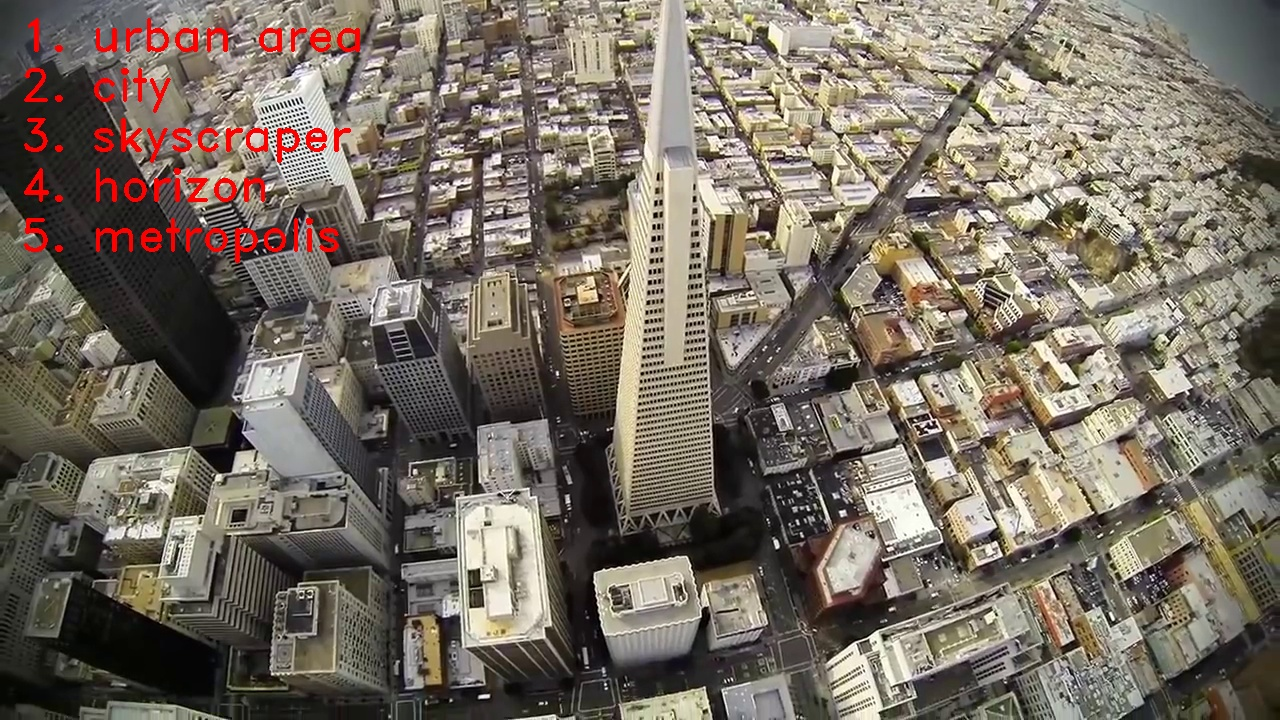
\includegraphics[width=1\textwidth]{/15.jpg}
\caption[Análisis de imagen tomada en una metrópoli]{Análisis de imagen tomada en una metrópoli}
\label{fig:imagen5}
\end{center}
\end{figure}

\begin{figure}[!h]
\begin{center}
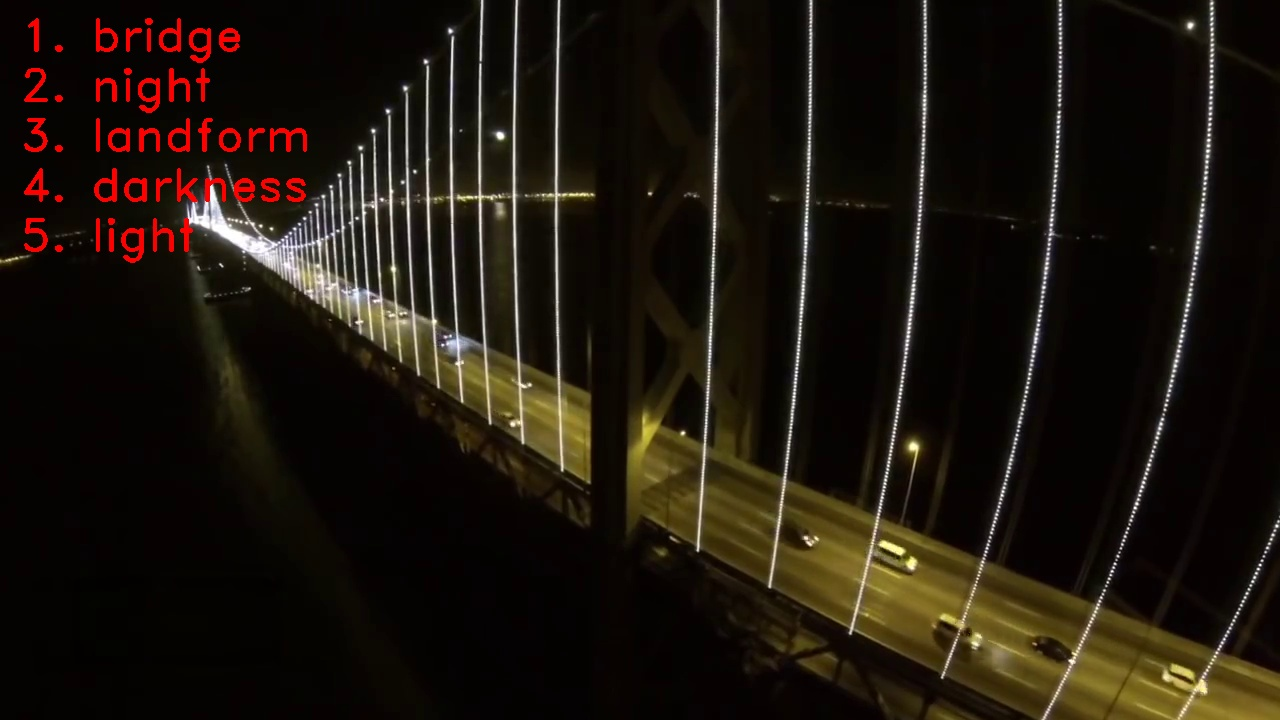
\includegraphics[width=1\textwidth]{/16.jpg}
\caption[Análisis de imagen tomada en un puente]{Análisis de imagen tomada en un puente}
\label{fig:imagen6}
\end{center}
\end{figure}

\begin{figure}[!h]
\begin{center}
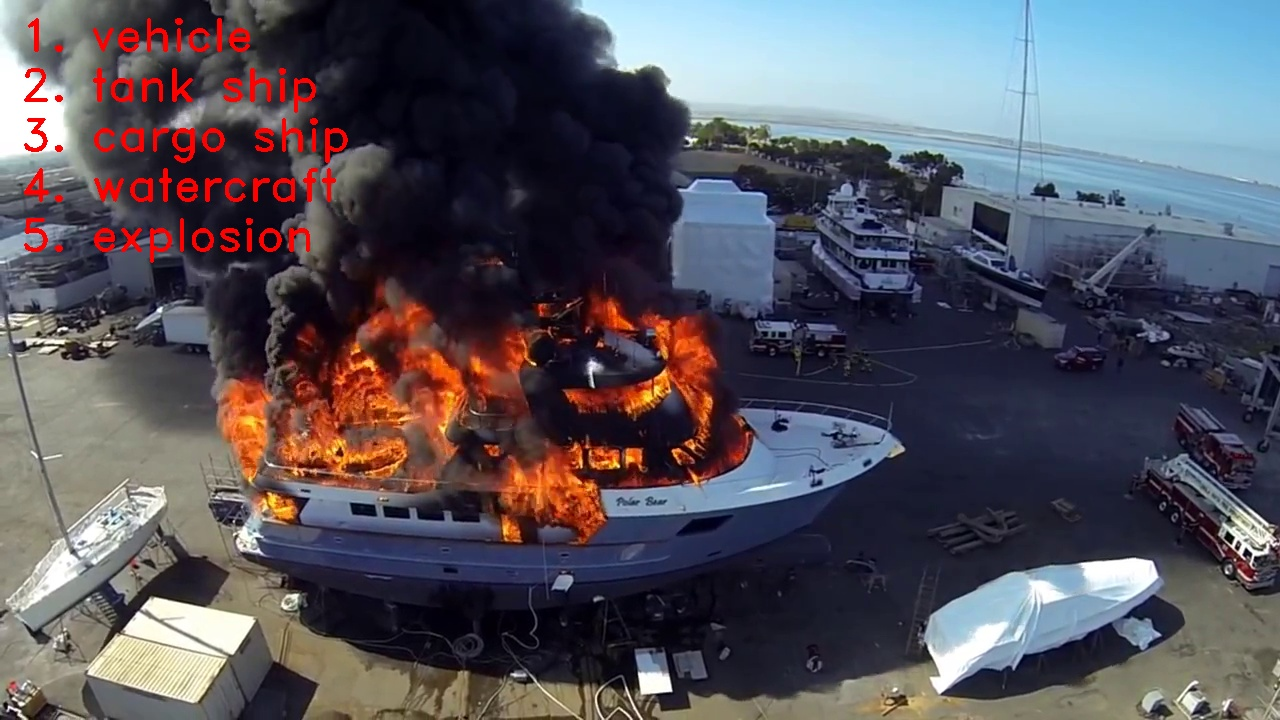
\includegraphics[width=1\textwidth]{/18.jpg}
\caption[Análisis de imagen de un barco incendiado]{Análisis de imagen de un barco incendiado}
\label{fig:imagen8}
\end{center}
\end{figure}

\begin{figure}[!h]
\begin{center}
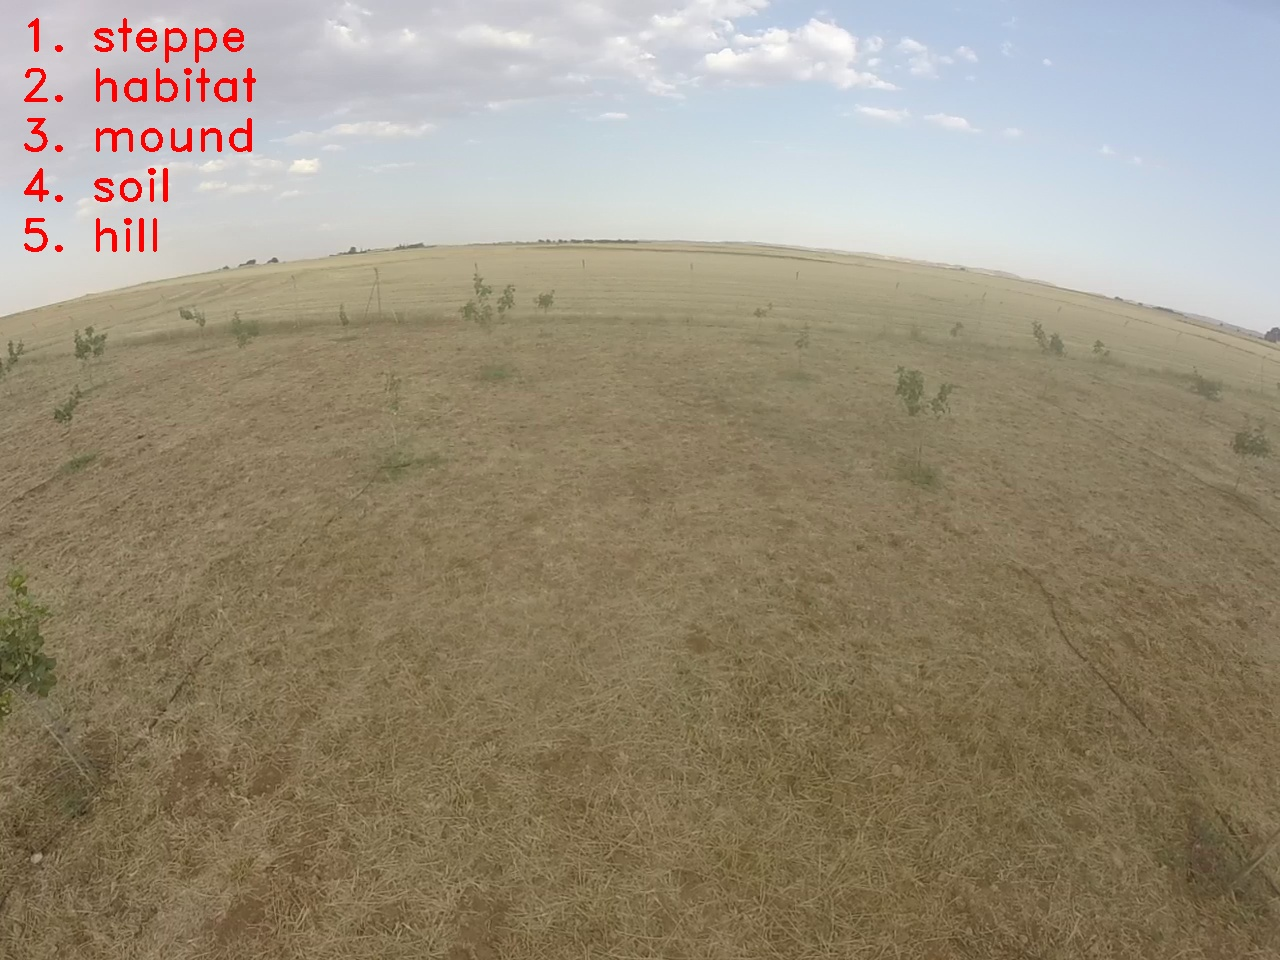
\includegraphics[width=1\textwidth]{/19.jpg}
\caption[Análisis de imagen tomada en el campo]{Análisis de imagen tomada en el campo}
\label{fig:imagen9}
\end{center}
\end{figure}


